\begin{multicols*}{2}
\section*{11. Heat Exchangers}
\subsection*{11.1. General Procedure}
\subsubsection*{11.1.1. Log Mean Temperature Difference Method}
\begin{enumerate}
    \item See if $\dot{Q}$ is given or can be obtained by energy balance
    \[ \dot{Q} = \dot{m} c_p (T_{\text{out},h} - T_{\text{in},h}) = \dot{m} c_p (T_{\text{in},c} - T_{\text{out},c}) \]
    \item Find the log mean temperature difference, $\Delta T_{\text{lm}}$
    \item Find the heat transfer coefficient, $U$, then profit
\end{enumerate}
\subsubsection*{11.1.2. $\varepsilon$-NTU Method}
\begin{enumerate}
    \item Find Rayleigh number, Ra$_L$, using fluid properties at average temperature $T_{\text{avg}} = (T_1 + T_2)/2$
    where $T_1$ and $T_2$ are the temperatures of the hot and cold surfaces respectively.
    \item Use the appropriate correlation to find the Nusselt number, Nu
    \item Determine the heat transfer coefficient $h$ using Nu, $k$, and $L_c$
\end{enumerate}
% Add this to a glossary section later
\subsection*{9.2. Variable Definitions}
\begin{itemize}
    \item $\dot{Q}$: Heat transfer rate
    \item $\dot{Q}_{\text{max}}$: Maximum heat transfer rate
    \item $T_{\text{in},h}$: Hot inlet temperature
    \item $T_{\text{out},h}$: Hot outlet temperature
    \item $T_{\text{in},c}$: Cold inlet temperature
    \item $T_{\text{out},c}$: Cold outlet temperature
    \item $U$: Overall heat transfer coefficient
    \item $\Delta T_{\text{lm}}$: Log mean temperature difference
    \item $F$: Correction factor 
    \item $\varepsilon$: Effectiveness
    \item $\dot{Q}_{\text{max}}$: Maximum heat transfer rate
    \item $C_c$: Cold heat capacity rate
    \item $C_h$: Hot heat capacity rate
    \item $c$: Heat capacity rate ratio
    \item $\text{NTU}$: Number of transfer units
\end{itemize}

\subsection*{11.3. Formulas}
\subsection*{11.3.1. Log Mean Temperature Difference Method}
For a heat exchanger,
\begin{align*}
    \dot{Q} &= \dot{Q}_{c} = -\dot{Q}_{h} 
\end{align*}
Overall heat transfer coefficient,
\begin{align*}
    \frac{1}{U A_s} &= \frac{1}{U_i A_{s,i}} = \frac{1}{U_o A_{s,o}} = R = \frac{1}{h_i A_{s,i}} +
    R_{\text{wall}} + \frac{1}{h_o A_{s,o}} 
\end{align*}
Log mean temperature difference,
\begin{align*}
    \Delta T_{\text{lm}} &= \frac{\Delta T_1 - \Delta T_2}{\ln(\Delta T_1 / \Delta T_2)} \\
    \Delta T_1 &= T_{\text{in},h} - T_{\text{out},c} \\
    \Delta T_2 &= T_{\text{out},h} - T_{\text{in},c} \\
    \dot{Q} &= U A_s \Delta T_{\text{lm}} 
\end{align*}
Correction factor,
\begin{align*}
    \Delta T_{\text{lm}} &= F \Delta T_{\text{lm, CF}} 
\end{align*}
where $\Delta T_{\text{lm, CF}}$ is the log mean temperature difference for counterflow and $F$ is the correction factor
which can be found in Figure \ref{fig:sec11_correction_factor}.

\subsection*{11.3.2. $\varepsilon$-NTU Method}
\begin{align*} 
    C_{\text{min}} &= \min(\dot{m}_c c_{p,c}, \dot{m}_h c_{p,h}) \\
    \dot{Q}_{\text{max}} &= C_{\text{min}} (T_{\text{in},h} - T_{\text{in},c}) \\
    \epsilon &= \frac{\dot{Q}}{\dot{Q}_{\text{max}}} \\
\end{align*}
if $C_c = C_{\text{min}}$,
\begin{align*}
    \epsilon &= \frac{\dot{Q}}{\dot{Q}_{\text{max}}} = \frac{T_{\text{out}, c} - T_{\text{in}, c}}{T_{\text{in}, h} - T_{\text{in}, c}} 
\end{align*}
if $C_h = C_{\text{min}}$,
\begin{align*}
    \epsilon &= \frac{\dot{Q}}{\dot{Q}_{\text{max}}} = \frac{T_{\text{in}, h} - T_{\text{out}, h}}{T_{\text{in}, h} - T_{\text{in}, c}}
\end{align*}
NTU is defined as,
\begin{align*}
    \text{NTU} &= \frac{UA_{s}}{C_{\text{min}}} = \frac{UA_{s}}{\dot{m} c_{p, \text{min}}} \\
    c &= \frac{C_{\text{min}}}{C_{\text{max}}} 
\end{align*}
The effectiveness, $\varepsilon$, can be found using Table \ref{tab:sec11_effectiveness_relations}.



\end{multicols*}
    
\section*{Tables}
\begin{figure}[H]
    \centering
    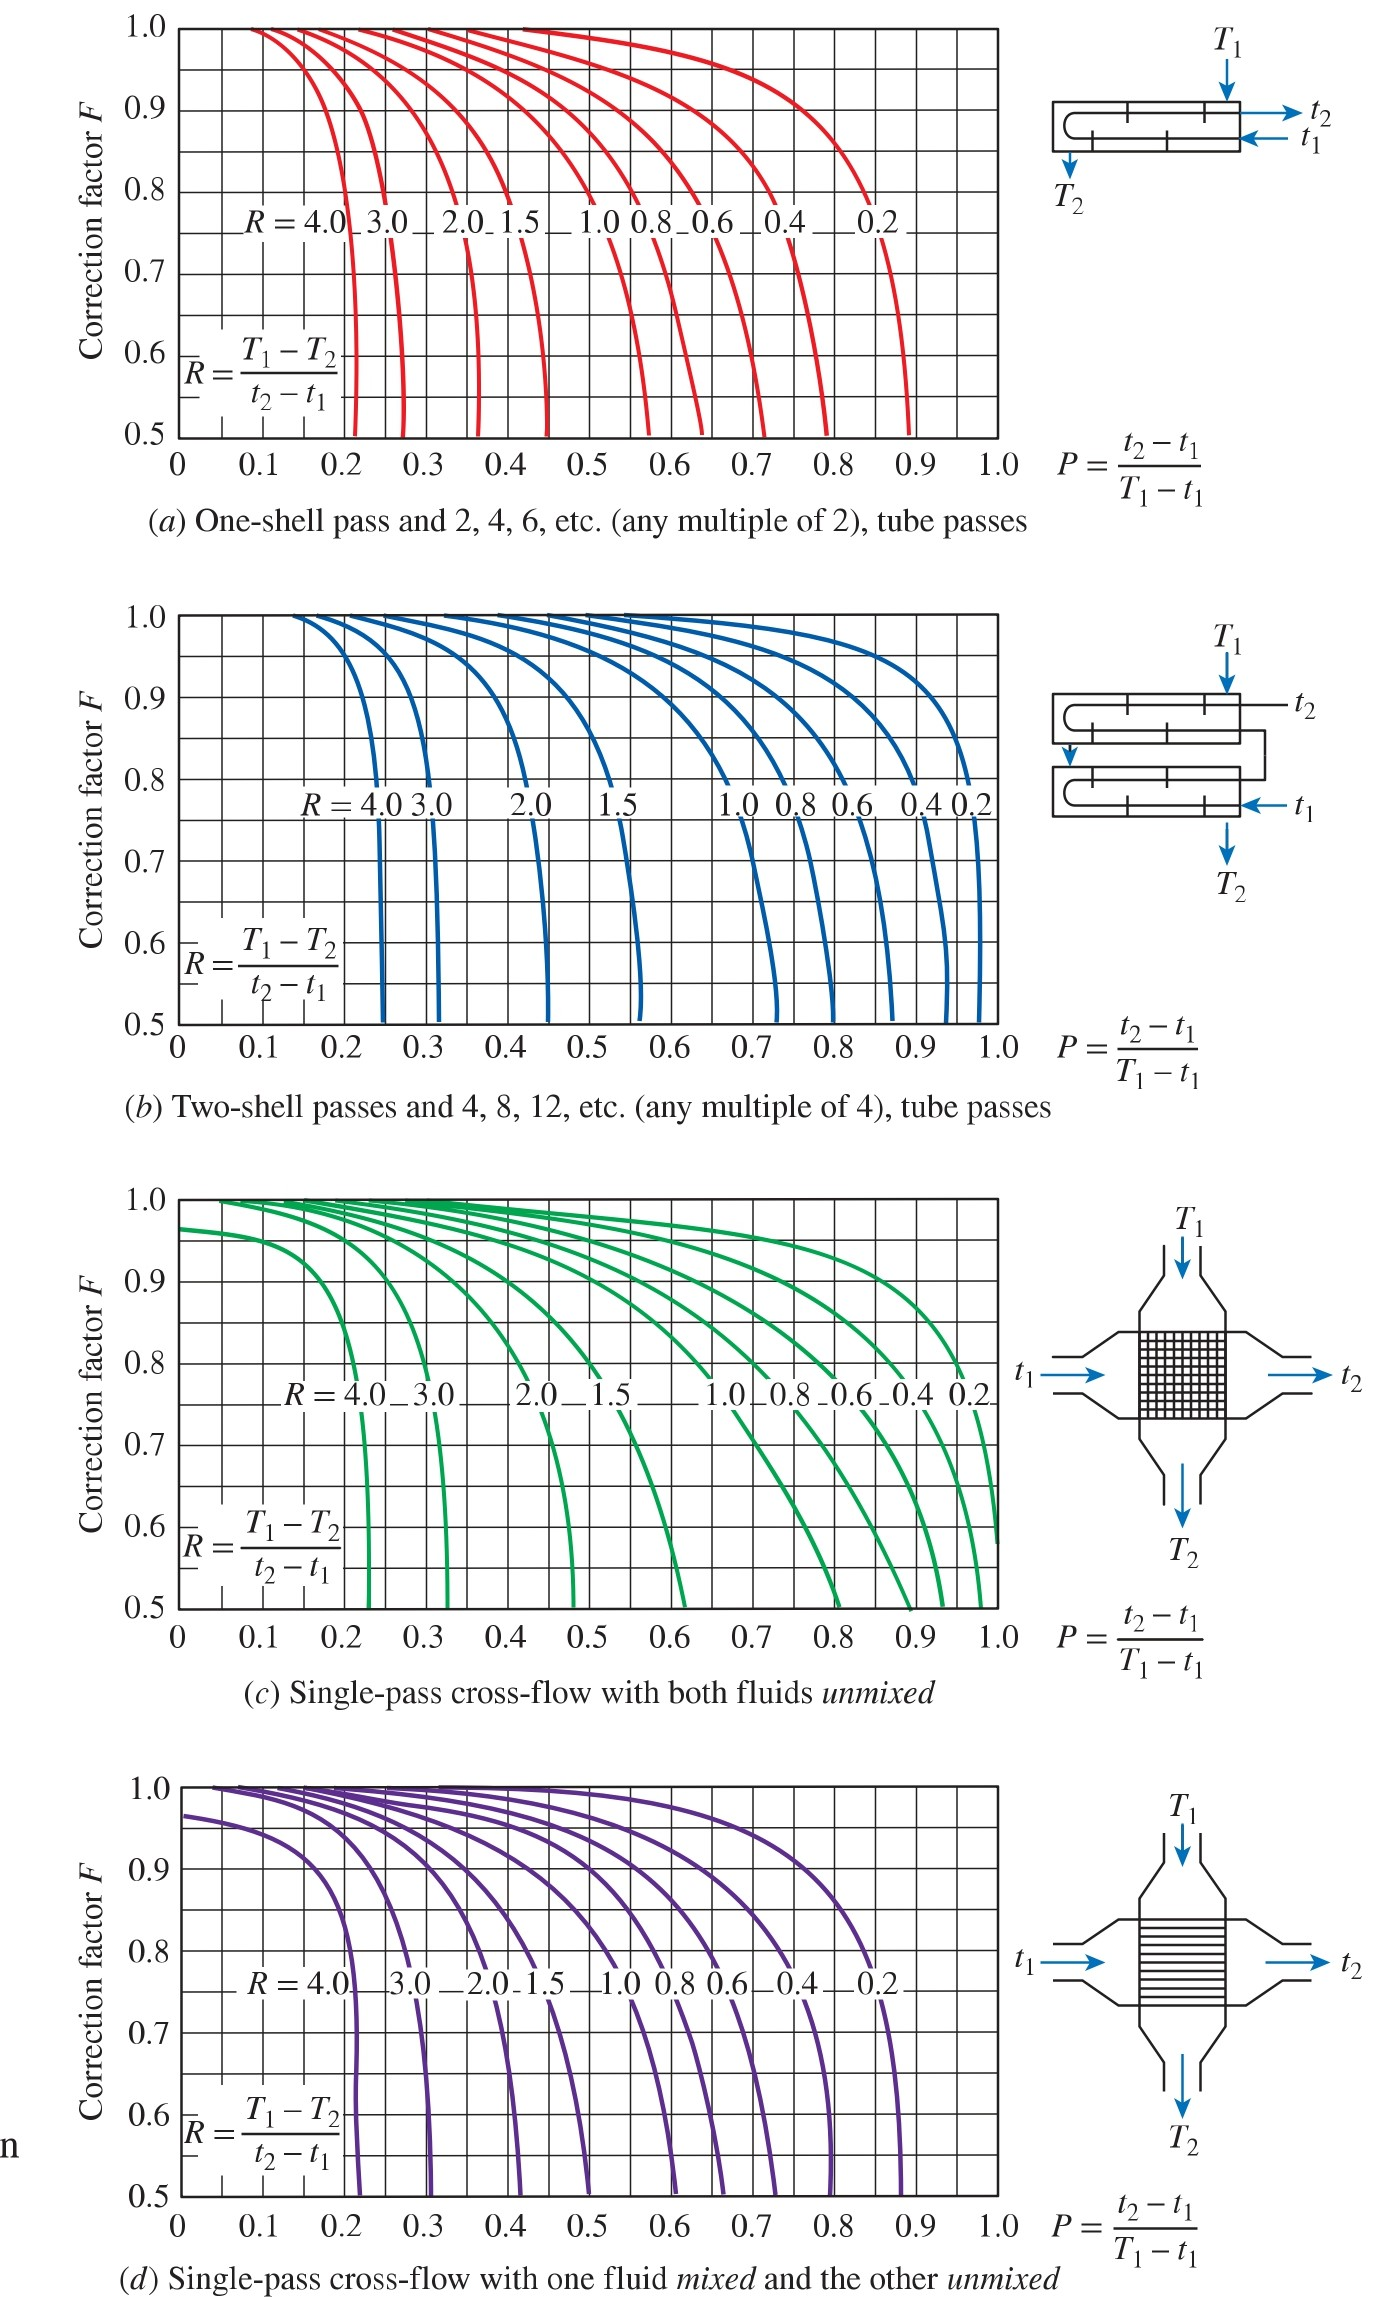
\includegraphics[width=0.7\linewidth]{Figures/Sec11 11-9.jpg}
    \caption{Correction factor F charts for common 
    shell-and-tube and crossflow heat 
    exchangers.}
    \label{fig:sec11_correction_factor}
\end{figure}
\newpage
\begin{table}[H]
    \centering
    \caption{Effectiveness relations for heat exchangers: NTU = $UA_s/C_{\text{min}}$ and $c = C_{\text{min}}/C_{\text{max}} =
    (\dot{m} c_p)_{\text{min}}/(\dot{m} c_p)_{\text{max}}$}
    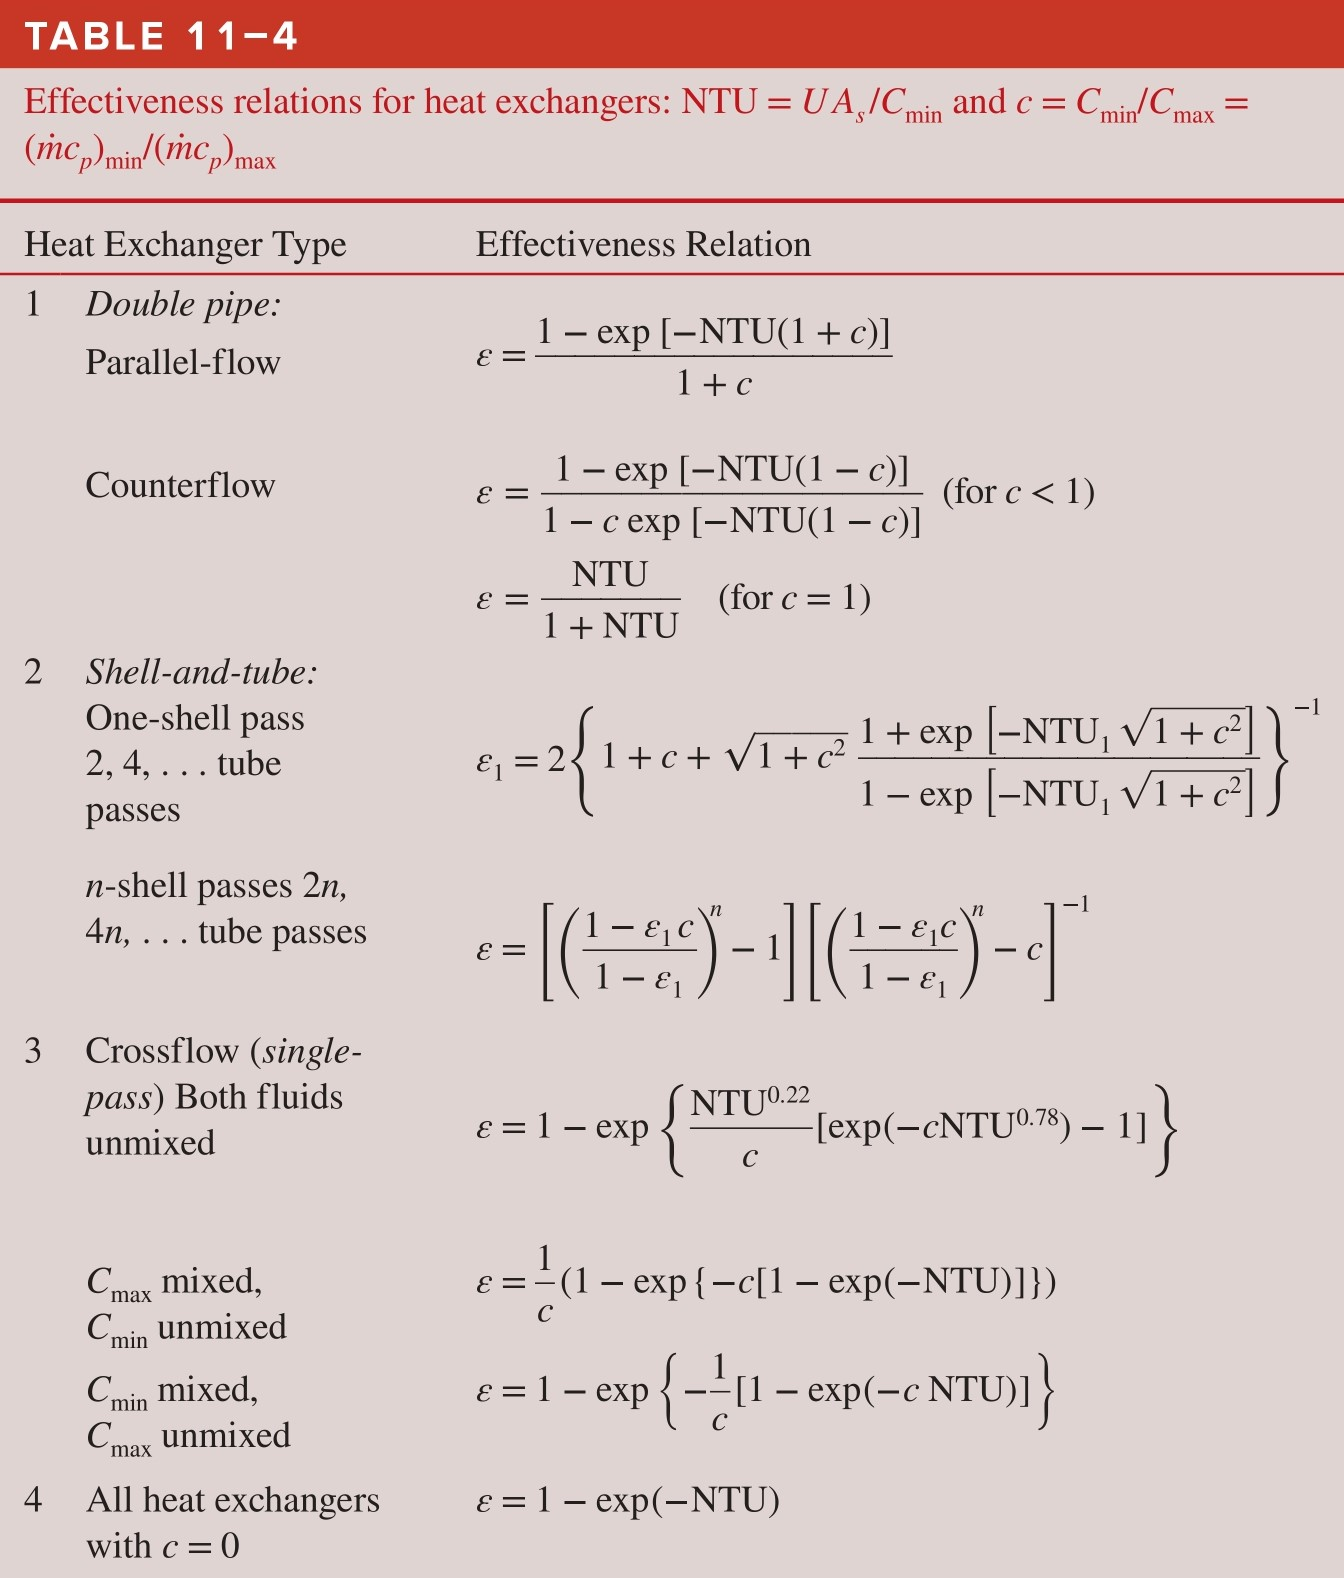
\includegraphics[width=0.8\linewidth]{Figures/Sec11 table 11-4.jpg}
    \label{tab:sec11_effectiveness_relations}
\end{table}
    